\documentclass[aspectratio=169,usenames,dvipsnames]{beamer}

\usetheme{default}  % You can choose any other theme you prefer

\title{04 - Algoritmos}
\author{Mateus Oliveira de Figueiredo}
\date{26/09/2023}

\usepackage{tikz}
\usepackage{multicol}
\usepackage{algorithm}
\usepackage{algpseudocode}
\usepackage{xcolor}
\usepackage[utf8]{inputenc}

\usepackage{pgfplots}
\DeclareUnicodeCharacter{2212}{−}
\usepgfplotslibrary{groupplots,dateplot}
\usetikzlibrary{patterns,shapes.arrows, positioning}
\pgfplotsset{compat=newest}

\begin{document}

\begin{frame}
\titlepage
\end{frame}

\begin{frame}
  \frametitle{Problema}

  \onslide<1->{
      Dado um conjunto de pontos no  $\mathbb{R}^2$, encontrar o menor conjunto convexo que contém todos os pontos (fecho convexo).
  }
  \begin{figure}
    \begin{overprint}
      \onslide<1> \begin{center}
% This file was created with tikzplotlib v0.10.1.
\begin{tikzpicture}[scale=0.9]

\definecolor{darkslategray38}{RGB}{38,38,38}
\definecolor{lightgray204}{RGB}{204,204,204}
\definecolor{steelblue76114176}{RGB}{76,114,176}

\begin{axis}[
axis line style={lightgray204},
hide x axis,
hide y axis,
tick align=outside,
x grid style={lightgray204},
xmajorticks=false,
xmin=0.0669367338947019, xmax=0.894111789939664,
xtick style={color=darkslategray38},
y grid style={lightgray204},
ymajorticks=false,
ymin=-0.0362471743023485, ymax=1.03274876525929,
ytick style={color=darkslategray38}
]
\addplot [draw=steelblue76114176, fill=steelblue76114176, mark=*, only marks]
table{%
x  y
0.346517060199814 0.201667385571862
0.110198245014805 0.710446973195645
0.674196381095166 0.49152149407659
0.30956117598126 0.80506608165215
0.271019344924566 0.98415804073376
0.636154602711755 0.693008958661624
0.384544745815431 0.621686927298183
0.613069361293463 0.536676532843469
0.515872695614497 0.0123435502231805
0.856512923755802 0.429885536698643
0.794765500051758 0.575905243509799
0.104535600078564 0.331190264339077
0.698107527894101 0.591287819523784
0.652331867510728 0.829843579751645
0.776100950068952 0.0753407526360956
0.359461819254946 0.832493157115646
0.234215740614521 0.440279847038206
0.474800803395323 0.180277096021146
0.478504950884847 0.867281705269675
0.434092000130053 0.504691515965982
0.640277876553855 0.402360080889356
};
\end{axis}

\end{tikzpicture}

\end{center}
      \onslide<2> % This file was created with tikzplotlib v0.10.1.
\begin{center}
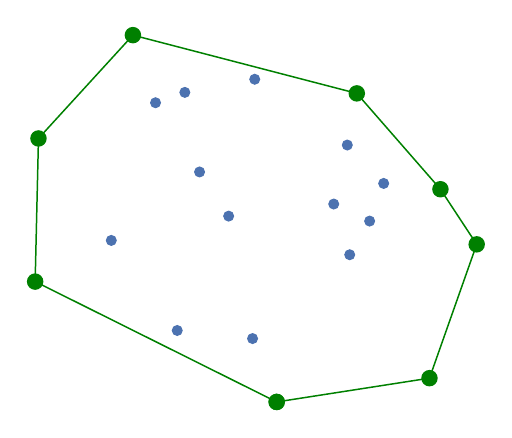
\begin{tikzpicture}[scale=0.9]

\definecolor{darkslategray38}{RGB}{38,38,38}
\definecolor{green}{RGB}{0,128,0}
\definecolor{lightgray204}{RGB}{204,204,204}
\definecolor{steelblue76114176}{RGB}{76,114,176}

\begin{axis}[
axis line style={lightgray204},
hide x axis,
hide y axis,
tick align=outside,
x grid style={lightgray204},
xmajorticks=false,
xmin=0.0669367338947019, xmax=0.894111789939664,
xtick style={color=darkslategray38},
y grid style={lightgray204},
ymajorticks=false,
ymin=-0.0362471743023485, ymax=1.03274876525929,
ytick style={color=darkslategray38}
]
\addplot [draw=steelblue76114176, fill=steelblue76114176, mark=*, only marks]
table{%
x  y
0.346517060199814 0.201667385571862
0.110198245014805 0.710446973195645
0.674196381095166 0.49152149407659
0.30956117598126 0.80506608165215
0.271019344924566 0.98415804073376
0.636154602711755 0.693008958661624
0.384544745815431 0.621686927298183
0.613069361293463 0.536676532843469
0.515872695614497 0.0123435502231805
0.856512923755802 0.429885536698643
0.794765500051758 0.575905243509799
0.104535600078564 0.331190264339077
0.698107527894101 0.591287819523784
0.652331867510728 0.829843579751645
0.776100950068952 0.0753407526360956
0.359461819254946 0.832493157115646
0.234215740614521 0.440279847038206
0.474800803395323 0.180277096021146
0.478504950884847 0.867281705269675
0.434092000130053 0.504691515965982
0.640277876553855 0.402360080889356
};
\addplot [semithick, green, mark=*, mark size=3, mark options={solid}]
table {%
0.515872695614497 0.0123435502231805
0.776100950068952 0.0753407526360956
0.856512923755802 0.429885536698643
0.794765500051758 0.575905243509799
0.652331867510728 0.829843579751645
0.271019344924566 0.98415804073376
0.110198245014805 0.710446973195645
0.104535600078564 0.331190264339077
0.515872695614497 0.0123435502231805
};
\end{axis}

\end{tikzpicture}
\end{center}
    \end{overprint}
  \end{figure}
\end{frame}

\begin{frame}{Algoritmo de Graham}
  % Make 2 columns
  \begin{columns}
    \begin{column}{0.5\textwidth}
      \begin{itemize}
        \onslide<1->{\item Encontrar o ponto mais baixo e a esquerda (pivot)}
        \onslide<3->{\item Ordena os pontos em ordem crescente de ângulo em relação ao pivot}
        \onslide<6->{\item Adiciona os pontos ao fecho convexo, caso não vire para a direita. Caso contrário, remove o ponto anterior.}
      \end{itemize}
    \end{column}
    \begin{column}{0.5\textwidth}
      \definecolor{green}{RGB}{0,128,0}
  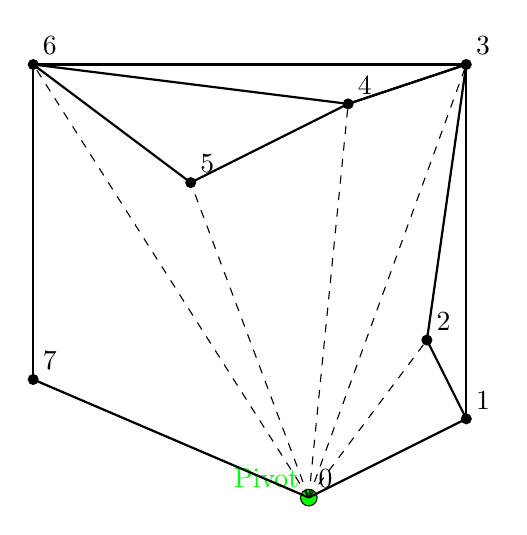
\begin{tikzpicture}
    % Define the points
    \coordinate (A) at (4,0);
    \coordinate (B) at (6,1);
    \coordinate (C) at (5.5, 2);
    \coordinate (D) at (6, 5.5);
    \coordinate (E) at (4.5, 5);
    \coordinate (F) at (2.5, 4.0);
    \coordinate (G) at (0.5, 5.5);
    \coordinate (H) at (0.5, 1.5);
    
    % Draw the points
    \foreach \point in {A,B,C,D,E,F,G,H}
      \fill (\point) circle (2pt);

    % Mark the pivot point
    \onslide<2->{
    \draw[fill=green] (A) circle (3pt);
    \node[above left, green] at (A) {Pivot};
    }

    % Draw a dashed line between the pivot and the points
    \onslide<3-4>{
        \draw[dashed] (A) -- (B);
        \draw[dashed] (A) -- (C);
        \draw[dashed] (A) -- (D);
        \draw[dashed] (A) -- (E);
        \draw[dashed] (A) -- (F);
        \draw[dashed] (A) -- (G);
        \draw[dashed] (A) -- (H);
    }
    
    % Label the points
    \onslide<4->{
        \node[above right] at (A) {0};
        \node[above right] at (B) {1};
        \node[above right] at (C) {2};
        \node[above right] at (D) {3};
        \node[above right] at (E) {4};
        \node[above right] at (F) {5};
        \node[above right] at (G) {6};
        \node[above right] at (H) {7};
    }

    \onslide<5->{
        \draw[thick] (A) -- (B);
    }

    \onslide<6-7>{
        \draw[thick] (B) -- (C);
    }

    \onslide<7>{
        \draw[thick] (C) -- (D);
    }

    \onslide<8->{
        \draw[thick] (B) -- (D);
    }

    \onslide<9-10>{
        \draw[thick] (D) -- (E);
        \draw[thick] (E) -- (F);
    }

    \onslide<10>{
        \draw[thick] (F) -- (G);
    }

    \onslide<11>{
        \draw[thick] (D) -- (E);
        \draw[thick] (E) -- (G);
    }

    \onslide<12->{
        \draw[thick] (D) -- (G);
    }

    \onslide<13->{
        \draw[thick] (G) -- (H);
    }

    \onslide<14->{
        \draw[thick] (H) -- (A);
    }


    
    % Draw the convex hull
    
    % Draw the convex hull
    % \draw[thick] (A) -- (C) -- (D) -- (F) -- (B) -- cycle;
    
    % Arrows indicating the convex hull construction
    % \draw[->, thick, red] ($(A)!0.5!(B)$) -- ($(A)!0.5!(C)$);
    % \draw[->, thick, red] ($(A)!0.5!(C)$) -- ($(A)!0.5!(D)$);
    % \draw[->, thick, red] ($(A)!0.5!(D)$) -- ($(A)!0.5!(F)$);
    % \draw[->, thick, red] ($(A)!0.5!(F)$) -- ($(A)!0.5!(B)$);
  \end{tikzpicture}

    \end{column}
  \end{columns}
  
\end{frame}

\begin{frame}{Exemplos}
  \begin{overprint}
    \begin{columns}
      \begin{column}{0.5\textwidth}
        \begin{figure}
          \includegraphics<1-2>[width=\textwidth]{./figures/cartbs_pointsonly.png}
          \includegraphics<3-4>[width=\textwidth]{./figures/catholebs_pointsonly.png}
          \includegraphics<5-6>[width=\textwidth]{./figures/dog_pointsonly.png}
        \end{figure}
      \end{column}
      \begin{column}{0.5\textwidth}
        \begin{figure}
          \includegraphics<2>[width=\textwidth]{./figures/cartbs.png}
          \includegraphics<4>[width=\textwidth]{./figures/catholebs.png}
          \includegraphics<6>[width=\textwidth]{./figures/dog.png}
        \end{figure}
      \end{column}
    \end{columns}
  \end{overprint}
\end{frame}

\begin{frame}{Algoritmos de Ordenação}

  \vfill

  Algoritmos $O(n^2)$ (pior caso):
  \begin{itemize}
    \item Selection Sort
    \item Insertion Sort
    \item Quick Sort - {\color{red} $O(n log(n))$ (caso médio)}
  \end{itemize}

  \vfill

  Algoritmos $O(n log(n))$ (pior caso):
  \begin{itemize}
    \item Merge Sort
    \item Heap Sort
  \end{itemize}

  \vfill
  
\end{frame}

\begin{frame}
\frametitle{Tempo de execução}
% Two columns
\begin{columns}
  \begin{column}{0.4\textwidth}
  \begin{itemize}
    \item Pontos gerados aleatoriamente dentro de um círculo de raio 1
    \item $h \sim \sqrt{n}$, onde h é o número de vértices do fecho convexo.
  \end{itemize}
  \end{column}
  \begin{column}{0.6\textwidth}
    \begin{figure}
      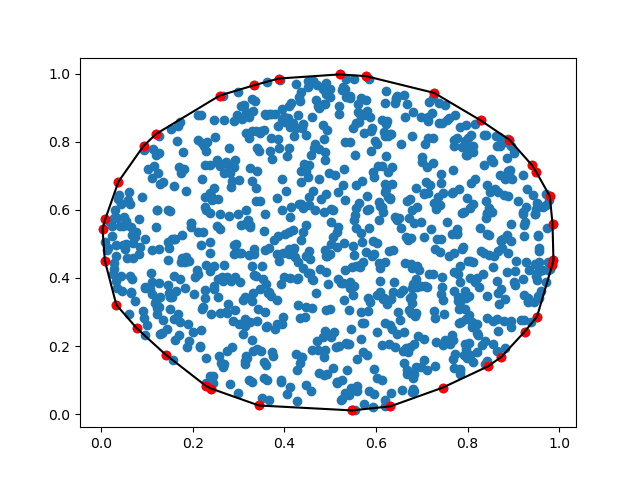
\includegraphics[width=0.9\textwidth]{./figures/random_merge_1000_1.png}
    \end{figure}
  \end{column}
\end{columns}
  
\end{frame}

\begin{frame}
\frametitle{Tempo de execução}
    \begin{figure}
        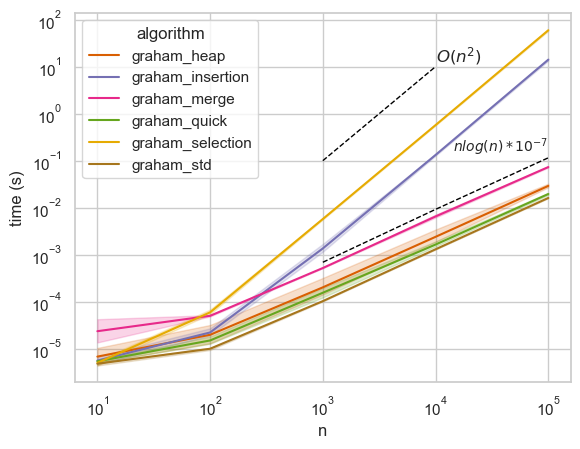
\includegraphics[width=0.7\textwidth]{./figures/circle_times.png}
    \end{figure}
\end{frame}

\begin{frame}
\frametitle{Tempo de execução}
    \begin{figure}
        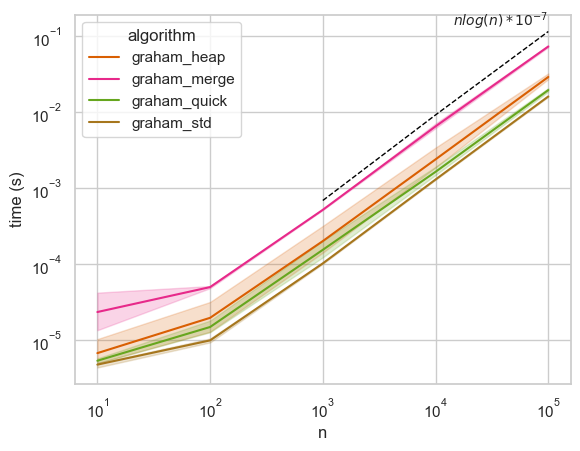
\includegraphics[width=0.7\textwidth]{./figures/circle_times_nlogn.png}
    \end{figure}
\end{frame}

\begin{frame}
\frametitle{Tempo de execução - Graham x Jarvis}
    \begin{figure}
      % include pgf circle_times.pgf here
      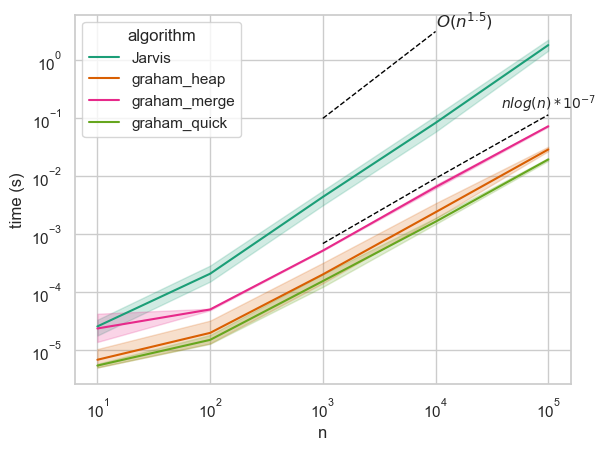
\includegraphics[width=0.7\textwidth]{./figures/circle_times_2.png}
    \end{figure}
\end{frame}


\end{document}
